\documentclass[12pt,a4paper]{article}
\usepackage[utf8]{inputenc}
\usepackage{amsmath}
\usepackage{amsfonts}
\usepackage{amssymb}
\usepackage{makeidx}
\usepackage{graphicx}
\usepackage{lmodern}
\usepackage{url}
\usepackage{bm}
\usepackage{booktabs}
\usepackage{float}
\usepackage[left=2cm,right=2cm,top=2cm,bottom=2cm]{geometry}
\author{Mudathir Mahgoub}
\title{Project report}
\begin{document}

\maketitle

\section{Summary of the original project pitch}

The project proposal was titled Cozmo/Vector Uber which attempts to simulate Uber service with cozmo and vector robots. In this simulation, the robot world is a small map with roads where robots navigate around without a purpose, until some one requests a trip through the mobile app. Then the closest robot selected by the app would complete the trip by moving from the starting point to the destination. The apps also enables monitoring the trip status and displaying robots movement on the map.  With this simulation, ``Robot Taxi" perhaps a better title than ``Cozmo/Vector Uber" because Uber supports shared taxi which is beyond the project 
scope. 

The project goals can be divided into 3 components described next. 

\subsection{Baseline goals for grade C} \label{sec:C}
The idea here is to implement the infrastructure needed for the simulation. The core of this infrastructure is a map with roads and buildings that is complex enough to support reasonable simulation. By reasonable simulation, I mean one that have multiple paths for the same trip to allow simple trip planning and shortest route computation. At the same time, the simulation doesn't need to be too complex to reflect the real world which would be too expensive, but abstract enough to capture the main component of Uber service. After some thinking I settled on the map shown in figure \ref{fig:proposedMap}. To build that map, lego road plates and buildings were suggested. 
\begin{figure}[H]
\center
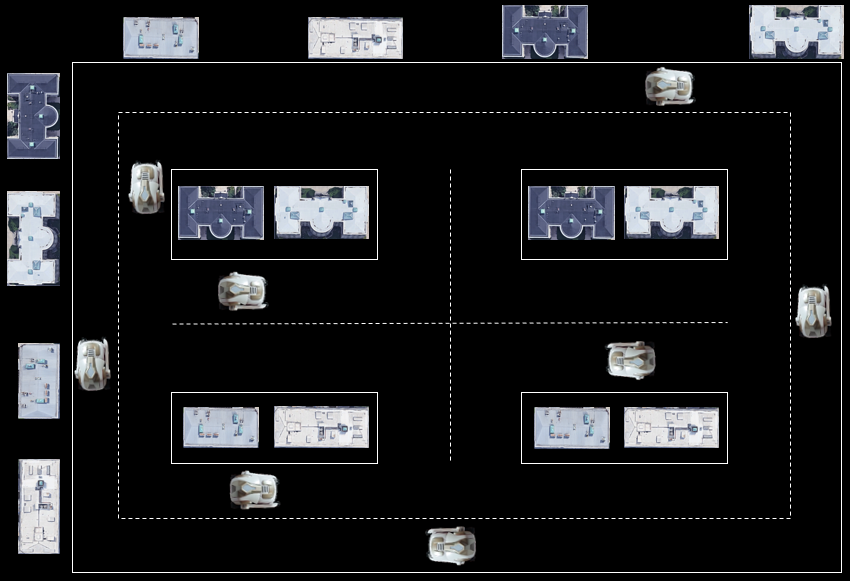
\includegraphics[scale=0.5]{./original_map.png}
\caption{The original proposed world.} \label{fig:proposedMap} 
\end{figure}


To implement the infrastructure for other components, the following goals were suggested: 

\begin{itemize}
\item Develop a server that assigns a new identifier to each connected robot client and monitors its current location

\item Develop a robot client that connects to the server and periodically sends its status and current location to the server

\item Develop a mobile app client which displays a map and the current locations of all robots connected to the server
\end{itemize}
\subsection{Additional components for grade B} \label{sec:B}

After implementing the infrastructure, the next step is to support trips. To do that, the following goals  were suggested:

\begin{itemize}
\item Add the feature of trip requests to the mobile app which enables the user to specify the starting point and destination point on the map. Unlike real world, in this world the mobile doesn’t have a GPS to detect its current location. The user can also specify the type of the robots: either spartan Cozmo or luxurious Vector. 

\item Add the trip planning feature to the server. For each trip request, the server identifies the nearest available robot and computes first the shortest route from the robot location to the  starting point, and then computes the shortest route from the starting point to the destination. The server then sends these routes to the selected robot

\item Update the robot client to receive a trip plan and execute it

\end{itemize}

\subsection{Top tier features for grade A} \label{sec:A}

To add some intelligence to the robot to avoid colliding with pedestrians and other robots,  the following goals were suggested:

\begin{itemize}
\item Build a neural network model to determine robot actions
\item Process images taken by the robot camera 
\item Stop all maneuvers if a person crossing the street is detected
\end{itemize}

\section{Evaluation of project progress}
Here is the story of the project progress since the proposal. 
\subsection{Building the map}
The original proposal for the map included buildings which would make the simulation pretty fancy. However, I After finding that the city buildings from Lego are too expensive, I moved them out of the project since they have little role in the implementation. Now that I reflect on project, perhaps these buildings would help in the deep learning by stopping the robots from going outside the roads. Also I could ask the kids in the family to build classic buildings from small pieces and bricks. 

For road plates I was looking for square turns to simplify the turns movements in corners. When I didn't find them I settled for rounded corners and the new map is shown in figure \ref{fig:map}.

\begin{figure}[H]
\center
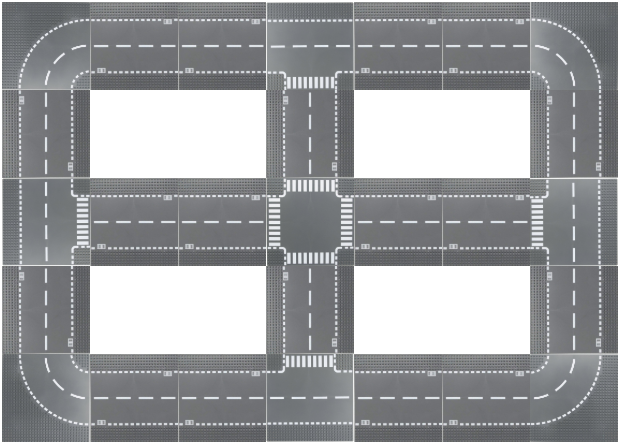
\includegraphics[scale=0.5]{./map.png}
\caption{The new world with empty white lands} \label{fig:proposedMap} 
\end{figure}

\subsection{Developing the server}
The natural next step after the map is to implement the server. Since the server plays a central role in the project and interacts with robots and mobile clients supporting different requests and responses, I chose Restful API approach with JSON to simplify the implementation. Since I was new to python, I looked for libraries that support Rest API and it seems Flask\footnote{\url{http://flask.pocoo.org/}} is a popular one. So I spent some time learning it and started implementing the server tasks. 

The first task was assigning new identity to each new robot (which simulates Uber driver and car registration in real life). The first challenge was storing the ids of the robots. In real life, I imagine Uber storing the registration information in a secure database. Since security and persistence  are not concerns in this project and database is overkill, I preferred to use the simple dictionary data struture in python to act as a storage for robots information. The next challenge was a consequence of using a dictionary. Since no primary key restriction is forced in the dictionary data structure, multiple robots can get the same id if their requests arrive at the same time. So I followed the basic mutex synchronization by using the lock objects provided by the threading library in python. 


Now that the server can assign a unique id to each robot, what comes next is to determine what to store in the dictionary. So I created a new class named \textbf{RobotState}:(\textit{robot\_id, robot\_type, x, y, rotation, update\_time}). Then I created server methods that supports getting and posting robot status, and created some unit tests to make sure that are working. 

\subsection{Developing the mobile client}

Now that the server supports simple features, the next step is to implement one of the clients: either the mobile client or the robot client. I decided to implement the mobile client first, since it is purely software which is faster than cozmo programming. Also implementing the mobile app would help me understand the requirements better, and clarify what is needed from robot clients. 

For the mobile app, I needed to display the map, locations of connected robots, and animation for their movements. At first I thought of implementing the mobile app on android devices. Then I remembered my experience with xbox controller in class where many students didn't participate because they had Mac laptops. So cross platforms compatibility is an issue.  Another issue was that cozmo already requires a mobile device, so I would need 2 android devices: one for cozmo and one for the mobile app which would make development painful and unnecessary complicated. Fortunately,  the solution to such problems is straightforward: developing a web page which is accessible by web browsers in all platforms including mobile devices. So it was time to refresh my rusty knowledge about javascript language. 


The first challenge I encountered, is how to draw maps and animations on a web page. My basic javascript skills didn't know how to do that then. So it was time again to look for libraries specialized on animation. The search result was D3 \footnote{\url{https://d3js.org/}} which stands for Data-Driven Documents. Its gallery\footnote{\url{https://github.com/d3/d3/wiki/Gallery}} looks very exciting with graphs, maps and animation. But I didn't know where to start from just the documentation. So I watched the online course \textit{d3-getting-started} from pluralsight\footnote{\textit{https://app.pluralsight.com/library/courses/d3-getting-started/table-of-contents}} to get started as its title says. After reading an article\footnote{\url{http://www.cagrimmett.com/til/2016/08/17/d3-lets-make-a-grid.html}} about drawing a grid using d3, I knew what to do and started coding. 


The first thing to draw was the map. To avoid hard coding the map, I created a Json file to store the map as cells. Each cell has the properties \textit{column, row, type, shape}. The cell type could be \textit{building} or \textit{road}. Since I am ignoring buildings their shapes don't matter. A road cell can have one of the following shapes: \textit{straightHorizontal, straightVertical, curveTopLeft, curveBottomLeft, curveBottomRigt, curveTopRight, tRight, tBottom, tLeft, tTop} and \textit{cross}.

Since web pages can't access files in the client machine, I made a special API for maps in the server so that the web page can retrieve the map when page content are loaded. When the map reached the web client, each cell gets drawn according to its type and shape. The next step is to draw some robots. 

\subsection{Developing the robot mock client}

After displaying the map on the web client, it is natural to implement cozmo client next. However I was reluctant to do that immediately for a couple of reasons: First I have only one cozmo, so I would only see one robot on the map if I implemented it first, Second cozmo development needs more time and configuration because it has hardware components and needs charging, third I would use 3 devices at the same time, Desktop, mobile and cozmo itself. So a \textit{mock client} that is purely software, simulates cozmo, doesn't need charging,  and requires only the desktop sounded very reasonable. 

Initially I ran multiple mock clients at once without movement. The web client displayed them correctly but it wasn't fun because no animation was involved. To do animation I had to implement random movements for the robot based on their current location. Since d3 uses CSS transitions for animation, I didn't need to implement movements on the pixel level. The cell level (which is 80 pixel) was enough for d3 to its magic. So all I needed is to move the mock robot from one road cell to a neighbor cell. Since backward movements and U-turns are not supported, the robot has at most 3 options depending on shape of its current cell: \textit{go straight}, \textit{turn right} or \textit{turn left}. 

For simplicity the mock client supports only 4 rotations: \textit{down} with rotation angle 0, \textit{up} with rotation down 180, \textit{right} with rotation angle 90, and \textit{left} with rotation \textit{180}. A challenge related to rotations was displaying them correctly using d3. Only \textit{down} rotation works perfectly. Other rotations are little off and it seems their geometric calculations need revisiting. With this, I thought I know what need to be done with the real client (cozmo client). How wrong I was is described next. 

\subsection{Developing the cozmo client}

Like the mock client, the plan for the cozmo client is to determine its current cell, randomly choose one of its neighbors, and choose the appropriate motor actions. However, I encountered a big problem: determining the current cell based on the position returned by cozmo  API was not accurate. 

It was really frustrating trying to navigate cozmo correctly on the map. First I tried controlling its wheels based on its positions, but that failed miserably. Then I tried computing the position myself following discrete movements to avoid positioning methods from cozmo API as follows:
\begin{itemize}
\item Start with \textit{current position} =$(x, y, rotation) = (0, 0, 0)$.
\item Use discrete actions to move cozmo to the next cell based on \textit{current position} which determines the \textit{current cell}. An example: 
\begin{enumerate}
\item $drive\_straight(distance)$
\item $turn\_in\_place(angle)$
\end{enumerate}

\item Update \textit{current cell} after completing the actions. After executing the above actions the \textit{current position} would be $(x, y, rotation) = (distance, 0, angle)$
\end{itemize}

This second approach also failed because  $turn\_in\_place(angle)$ was not reliable. I was stuck at this point, so I postponed cozmo client and decided to do other things in the project. Since section \ref{sec:B} depends on cozmo client, I focused on accomplishing the goals in section \ref{sec:A}. 

\subsection{Deep learning}

 Include your successes and failures, and an assessment of how you met your project goals.  If you ended up modifying your goals, provide those details as well.  If you worked with another student, highlight your contributions to the project.  This component should reflect your work on the project, and your evaluation of your project.  You should also include challenges you ran into related to programming Cozmo.  For example, if I were writing such a report, I might include a warning that Cozmo may require a firmware update (through the app) in order to run, and that this update might then require an update to the SDK, and this could happen without much warning.  This observation was inspired by my experience with running my back-to-back Cozmo workshops.  I am not trying to say that you need to include this in your report.  I am just trying to give you an example of something that I experienced that I would have included in my report.  If you had problems using a particular phone to connect to Cozmo, you might mention that in your report.  You are sharing these experiences because other people might encounter them and need help...  You are telling me the story of the development of your project in this section.

\section{Technical details}
Special packages that were needed in order to run your program.  Include clear set-up instructions if necessary.  For example, if your project involved using pygame or numpy, include the pip install commands to install those libraries.  You can assume that everyone is starting with having installed the Cozmo SDK, but there is no harm in explicitly mentioning that, as well as the lines to install or upgrade the SDK.  Assume that someone just learning to program in Python will be trying to replicate your work.  Screen shots are not necessary, but clear instructions are.  If your code only runs on Linux, be sure to specify that.  If your project requires a Virtual Box, or Matlab, or other ML components, be sure to include instructions on how to set those up.  You are providing technical details of your project in this section.

\subsection{programming details}

A link to the GitHub repository to access your code.  You are providing the programming details of your project in this section.

\section{Acknowledgements and Gratitude}

Acknowledgements and Gratitude: If you used someone else's code, or followed specific tutorials to solve problems, give those people/sources credit.  Provide links for useful resources that helped you, including DIY guides, tutorials, etc...  If someone in the class helped you address/solve problems, this would be the place to thank them.  If you benefitted from either the Dash Button or Xbox Controller activity, be sure to acknowledge that here as well.  We all benefit from the tech community, and should appreciate the shoulders of the giants who support us.  You are providing references in this section.


\bibliographystyle{plain}

\bibliography{references}

\end{document}
